\title{Introdução a Árvores (Estruturas de Dados)}
\date{\today}
\frame{\titlepage}

% Slide 1: Introdução às Árvores como Conceito
\begin{frame}[fragile]
  \frametitle{Introdução às Árvores como Conceito}
  \begin{itemize}
    \item \textbf{Definição:} Uma árvore, em ciência da computação, é uma estrutura de dados hierárquica que simula uma estrutura de árvore com um conjunto de nós conectados.
    \item \textbf{Raízes Biológicas:} Inspirado nas árvores da natureza, onde um tronco se ramifica em muitos galhos, que por sua vez podem se dividir em mais galhos, até chegar às folhas.
    \item \textbf{Aplicabilidade:} Árvores são essenciais para representar estruturas organizacionais, árvores genealógicas e em várias estruturas de dados como árvores binárias, árvores AVL, árvores de segmento, etc.
  \end{itemize}
\end{frame}

% Slide 2: Estruturas Organizacionais e Árvores Genealógicas
\begin{frame}[fragile]
  \frametitle{Estruturas Organizacionais e Árvores Genealógicas}
  \begin{itemize}
    \item \textbf{Estruturas Organizacionais:} Utilizam o conceito de árvores para representar hierarquias dentro de uma organização, desde o nível mais alto de gestão até os funcionários de nível base.
    \item \textbf{Árvores Genealógicas:} Mostram as relações de parentesco entre os membros de uma família ao longo de gerações, onde cada pessoa pode ser vista como um nó conectado aos seus ascendentes e descendentes.
    \item \textbf{Visualização:} Ambos os exemplos ajudam a entender a utilidade das árvores na organização e na representação de relações hierárquicas complexas.
  \end{itemize}
\end{frame}
\begin{frame}[fragile]
  \frametitle{Estruturas Organizacionais}
  \begin{figure}
    \centering
    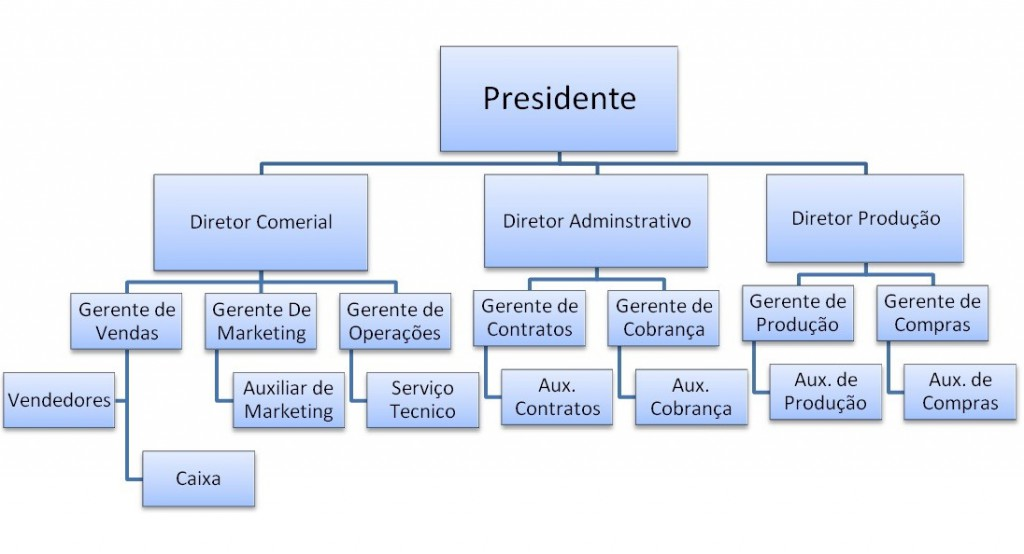
\includegraphics[width=0.7\textwidth]{assets/aula5-arvore-organograma.jpeg}
    \caption{Estruturas Organizacionais}
  \end{figure}
\end{frame}
\begin{frame}[fragile]
  \frametitle{Árvores Genealógicas}
  \begin{figure}
    \centering
    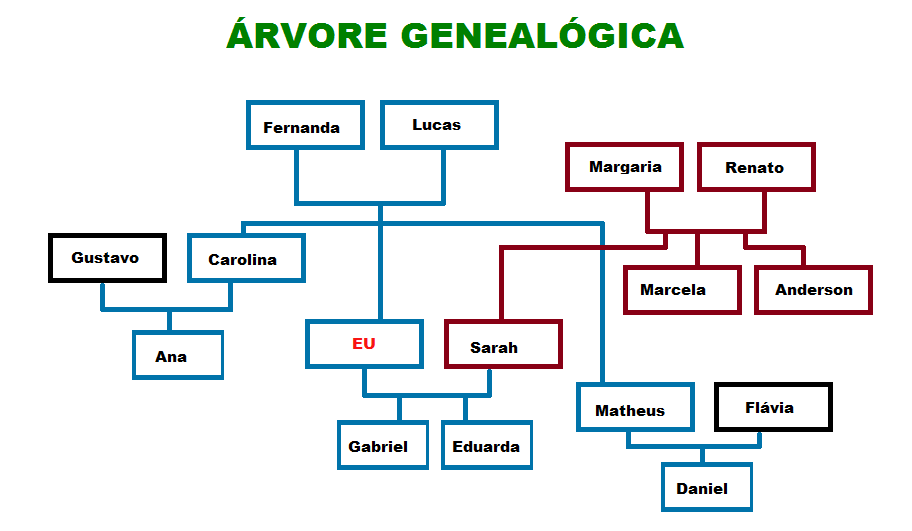
\includegraphics[width=0.7\textwidth]{assets/aula5-arvore-genealogica.png}
    \caption{Árvores Genealógicas}
  \end{figure}
\end{frame}
% Slide: Árvores de Decisão no Jogo da Velha
\begin{frame}[fragile]
  \frametitle{Árvores de Decisão no Jogo da Velha}
  \begin{itemize}
    \item \textbf{Conceito:} Uma árvore de decisão é um diagrama que representa decisões e seus possíveis resultados. No contexto de jogos, é usada para modelar as possibilidades de jogadas e seus desfechos.
    \item \textbf{Aplicação no Jogo da Velha:}
      \begin{itemize}
        \item Cada nó representa o estado atual do tabuleiro.
        \item Cada ramificação a partir de um nó representa uma jogada possível.
        \item Folhas da árvore representam o desfecho da partida (vitória, derrota ou empate).
      \end{itemize}
    \item \textbf{Utilização:} Árvores de decisão permitem a um algoritmo de IA antecipar movimentos, escolhendo o caminho que maximiza a chance de vitória ou minimiza a de derrota.
    \item \textbf{Desenvolvimento de Estratégias:} Analisando a árvore de decisão completa do jogo da velha, é possível desenvolver uma estratégia perfeita, onde a IA nunca perde, podendo no máximo empatar.
    \item \textbf{Implicações:} Este modelo é um exemplo fundamental de como técnicas simples de IA podem ser aplicadas para resolver problemas complexos em jogos e em outras áreas da computação.
  \end{itemize}
\end{frame}
\begin{frame}[fragile]
  \frametitle{Árvores de Decisão no Jogo da Velha}
  \begin{figure}
    \centering
    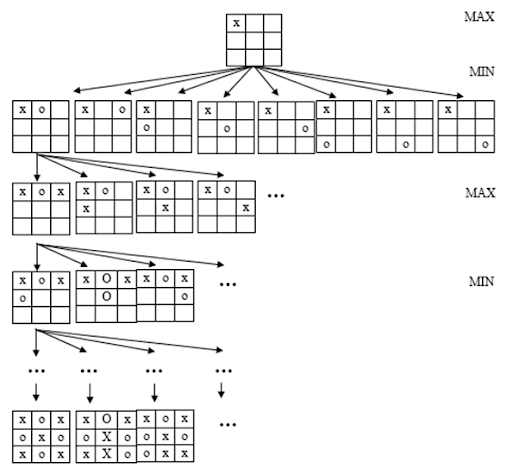
\includegraphics[width=0.7\textwidth]{assets/aula5-tic.png}
    \caption{Árvores de Decisão no Jogo da Velha}
  \end{figure}
\end{frame}


% Slide 3: Conceitos Básicos de Árvores em Estruturas de Dados
\begin{frame}[fragile]
  \frametitle{Conceitos Básicos de Árvores em Estruturas de Dados}
  \begin{itemize}
    \item \textbf{Nó:} Elemento básico que contém dados e links para outros nós (filhos).
    \item \textbf{Raiz:} Nó no topo da árvore, sem pais.
    \item \textbf{Folhas:} Nós sem filhos, localizados na base da árvore.
    \item \textbf{Altura:} Comprimento do caminho mais longo de um nó à uma folha.
  \end{itemize}
\end{frame}
\begin{frame}[fragile]
  \frametitle{Árvores em Estruturas de Dados}
  \begin{figure}
    \centering
    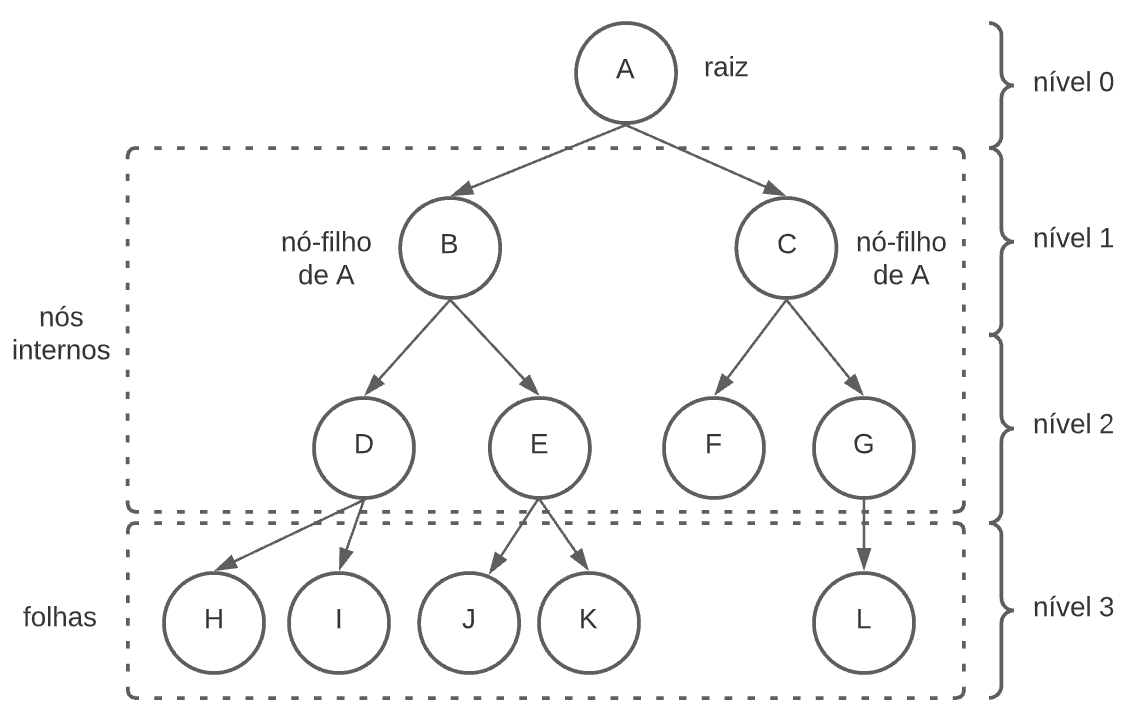
\includegraphics[width=0.7\textwidth]{assets/aula5-arvores1.png}
    \caption{Árvores em Estruturas de Dados}
  \end{figure}
\end{frame}

\begin{frame}[fragile]
  \frametitle{Inspecionando os elementos de uma árvore}
  \begin{figure}
    \centering
    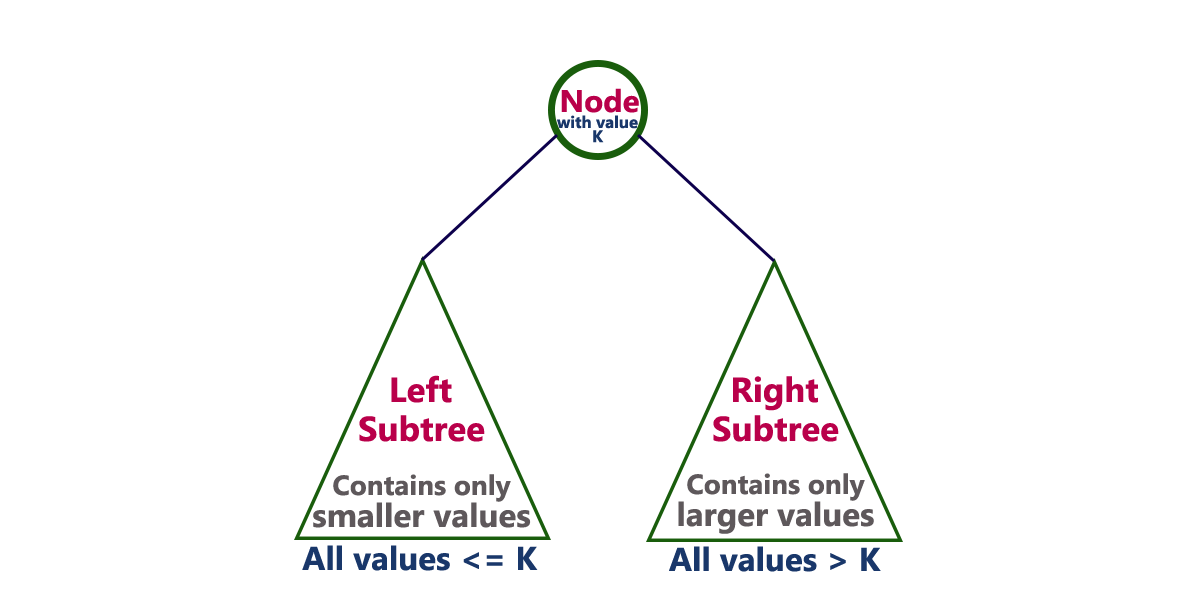
\includegraphics[width=0.5\textwidth]{assets/aula5-arvores3.png}
    \caption{Inspecionando os elementos de uma árvore}
  \end{figure}
\end{frame}
% Slide 4: Árvores Binárias e suas Operações
\begin{frame}[fragile]
  \frametitle{Árvores Binárias e suas Operações}
  \begin{itemize}
    \item \textbf{Definição:} Uma árvore binária é uma estrutura de árvore em que cada nó tem no máximo dois filhos, conhecidos como filho à esquerda e filho à direita.
    \item \textbf{Operações Principais:}
      \begin{itemize}
        \item \textit{Inserção:} Adiciona um novo nó na árvore na posição adequada.
        \item \textit{Remoção:} Remove um nó da árvore, mantendo as propriedades da árvore binária.
        \item \textit{Busca:} Encontra um valor dentro da árvore.
      \end{itemize}
    \item \textbf{Percursos:} Em ordem, pré-ordem e pós-ordem são métodos para visitar todos os nós de uma árvore binária.
  \end{itemize}
\end{frame}

% Slide 5: Aplicações Práticas de Árvores
\begin{frame}[fragile]
  \frametitle{Aplicações Práticas de Árvores}
  \begin{itemize}
    \item \textbf{Bancos de Dados:} Árvores B e árvores B+ são utilizadas em sistemas de gerenciamento de banco de dados para indexação e busca rápida de dados.
    \item \textbf{Gráficos de Computador:} Árvores são usadas em algoritmos de renderização para organizar e processar objetos em uma cena.
    \item \textbf{Redes:} Estruturas de árvore ajudam na organização e na otimização de redes, como em protocolos de roteamento.
    \item \textbf{Conclusão:} O estudo de árvores é fundamental na ciência da computação, com aplicações vastas e significativas em diversos campos.
  \end{itemize}
\end{frame}

\begin{frame}[fragile]
  \frametitle{Introdução às Árvores Binárias Não Balanceadas}
  \begin{itemize}
    \item \textbf{Definição:} Uma árvore binária não balanceada é uma estrutura de dados em que cada nó tem até dois filhos, mas sem garantias específicas sobre a altura da árvore, o que pode levar a desequilíbrios significativos no número de nós entre as subárvores esquerda e direita.
    \item \textbf{Propriedades:}
      \begin{itemize}
        \item Cada nó representa um elemento ou valor.
        \item Cada nó pode ter até dois filhos: um à esquerda e um à direita.
        \item Não há restrições específicas de balanceamento, permitindo que a árvore se torne assimétrica.
      \end{itemize}
    \item \textbf{Aplicabilidade:} Embora simples, as árvores binárias não balanceadas são fundamentais para entender conceitos mais avançados em estruturas de dados, como árvores balanceadas e árvores de busca.
  \end{itemize}
\end{frame}

\begin{frame}[fragile]
  \frametitle{Inspecionando os elementos de uma árvore}
  \begin{figure}
    \centering
    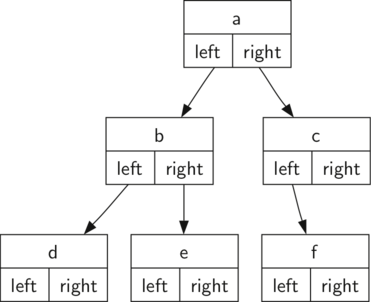
\includegraphics[width=0.5\textwidth]{assets/aula5-arvores2.png}
    \caption{Inspecionando os elementos de uma árvore}
  \end{figure}
\end{frame}
% Slide: Organização dos Nós
\begin{frame}[fragile]
  \frametitle{Organização dos Nós}
  \begin{itemize}
    \item \textbf{Regra Geral:}
      \begin{itemize}
        \item Nós à esquerda de um dado nó contêm valores menores.
        \item Nós à direita de um dado nó contêm valores maiores.
      \end{itemize}
    \item \textbf{Importância:} Esta organização facilita operações de busca, inserção e remoção, permitindo que operações como busca binária sejam realizadas eficientemente.
    \item \textbf{Exceções:} Em árvores binárias não necessariamente de busca, a organização dos nós pode seguir outras lógicas específicas, dependendo da aplicação.
  \end{itemize}
\end{frame}


\begin{frame}[fragile]
  \frametitle{Inspecionando os elementos de uma árvore}
  \begin{figure}
    \centering
    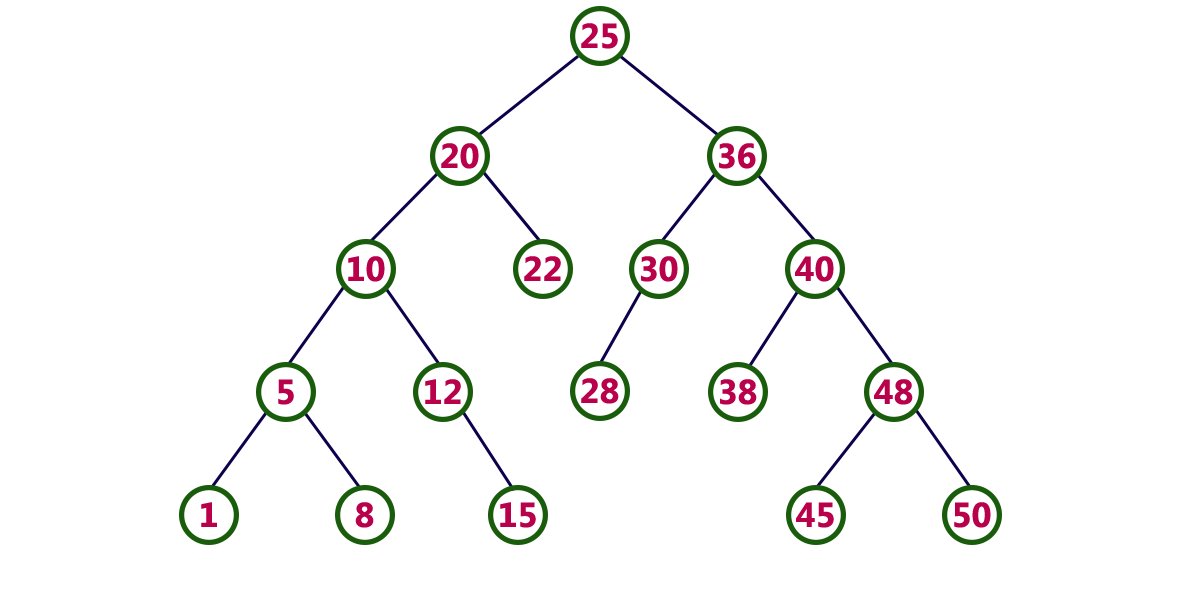
\includegraphics[width=0.5\textwidth]{assets/aula5-arvores4.png}
    \caption{Inspecionando os elementos de uma árvore}
  \end{figure}
\end{frame}
% Slide: Inserção em Árvores Binárias Não Balanceadas
\begin{frame}[fragile]
  \frametitle{Inserção em Árvores Binárias Não Balanceadas}
  \begin{itemize}
    \item \textbf{Processo de Inserção:}
      \begin{itemize}
        \item Iniciar no nó raiz.
        \item Comparar o valor a ser inserido com o valor do nó atual.
        \item Se o valor for menor, mover para o filho à esquerda; se maior, para o direito.
        \item Repetir o processo até encontrar um local vazio onde o novo nó possa ser inserido.
      \end{itemize}
    \item \textbf{Considerações:} Esse método de inserção mantém a propriedade fundamental da árvore binária, mas pode levar a uma árvore desequilibrada se os valores inseridos não estiverem em uma ordem aleatória.
    \item \textbf{Desafios:} A falta de balanceamento pode resultar em uma eficiência reduzida para operações de busca, inserção e remoção, especialmente em casos extremos onde a árvore se assemelha a uma lista encadeada.
  \end{itemize}
\end{frame}

\begin{frame}[fragile]
  \frametitle{Inspecionando os elementos de uma árvore}
  \begin{figure}
    \centering
    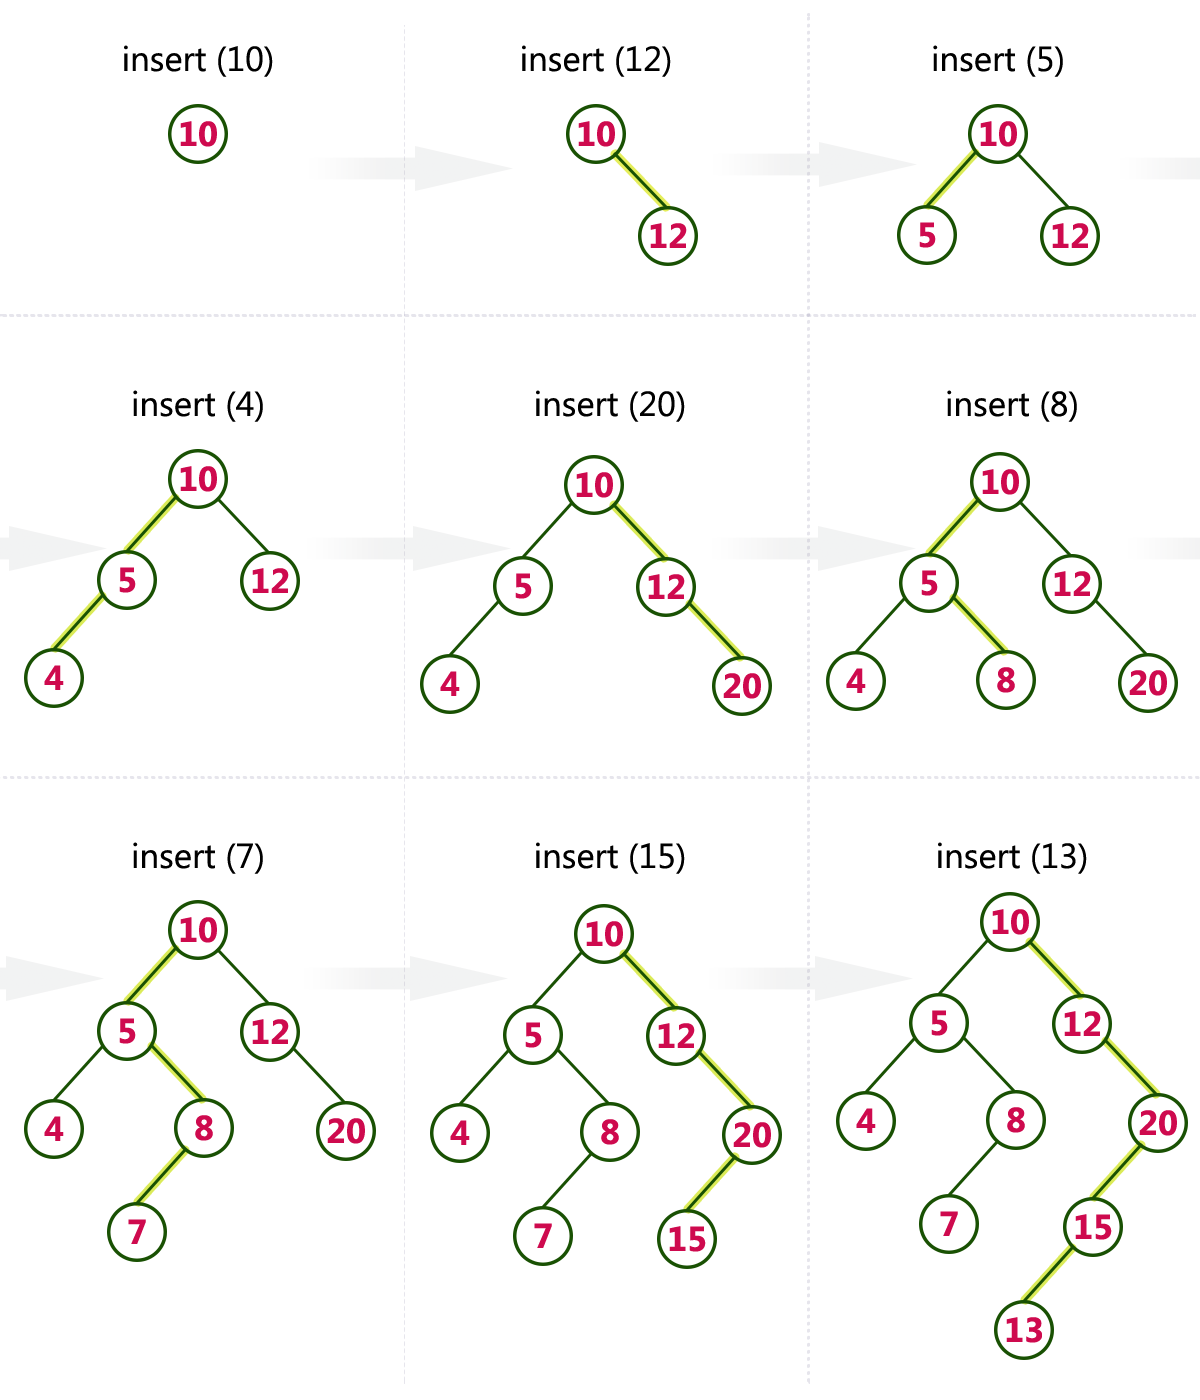
\includegraphics[width=0.4\textwidth]{assets/aula5-arvores5.png}
    \caption{Inspecionando os elementos de uma árvore}
  \end{figure}
\end{frame}
% Slide: Ordenação e Traversal
\begin{frame}[fragile]
  \frametitle{Ordenação e Traversal}
  \begin{itemize}
    \item \textbf{Traversal:} As árvores binárias suportam vários métodos de traversal (percurso), que determinam a ordem na qual os nós são visitados, incluindo:
      \begin{itemize}
        \item \textit{Preordem:} Visita primeiro a raiz, depois a subárvore esquerda, seguida da subárvore direita.
        \item \textit{Inordem:} Visita primeiro a subárvore esquerda, depois a raiz, e finalmente a subárvore direita
        \item \textit{Inordem:} Visita primeiro a subárvore esquerda, depois a raiz, e finalmente a subárvore direita. Este método resulta nos valores sendo visitados em ordem crescente, útil para obter os elementos da árvore ordenados.
        \item \textit{Pós-ordem:} Visita primeiro as subárvores esquerda e direita, e por último a raiz. É útil para operações que precisam processar um nó depois de seus descendentes, como liberar memória de uma árvore.
      \end{itemize}
  \end{itemize}
\end{frame}
% Slide: Ordenação e Traversal
\begin{frame}[fragile]
  \frametitle{Ordenação e Traversal}
  \begin{itemize}
    \item \textbf{Ordenação:}
      \begin{itemize}
        \item Através do traversal inordem, é possível extrair todos os elementos de uma árvore binária em ordem crescente.
        \item Este processo é especialmente útil para visualizar a estrutura de dados de uma maneira linear e ordenada, ou para realizar operações ordenadas sobre os dados.
      \end{itemize}
    \item \textbf{Importância do Traversal:} A escolha do método de traversal afeta diretamente a eficiência e o tipo de operações que podem ser realizadas em uma árvore. Por exemplo, o traversal inordem é essencial para operações de busca e ordenação, enquanto o pré-ordem e pós-ordem são importantes para reconstruir ou copiar a árvore.
  \end{itemize}
\end{frame}

% Slide: Exercício de Inserção em Árvores Binárias Não Balanceadas
\begin{frame}[fragile]
  \frametitle{Exercício de Inserção em Árvores Binárias Não Balanceadas}
  \begin{itemize}
    \item \textbf{Objetivo:} Praticar a inserção de valores em árvores binárias não balanceadas, observando como a estrutura da árvore se desenvolve com cada inserção.
    \item \textbf{Instruções:}
      \begin{enumerate}
        \item Comece com uma árvore vazia.
        \item Insira os valores do conjunto fornecido, um de cada vez, seguindo as regras de inserção para árvores binárias.
        \item Após cada inserção, desenhe a árvore resultante.
        \item Repita o processo para cada conjunto de valores fornecido.
      \end{enumerate}
  \end{itemize}
\end{frame}


% Slide: Exercício de Inserção em Árvores Binárias Não Balanceadas
\begin{frame}[fragile]
  \frametitle{Exercício de Inserção em Árvores Binárias Não Balanceadas}
  \begin{itemize}
    \item \textbf{Conjuntos de Valores:}
      \begin{itemize}
        \item \textit{Conjunto 1:} 11, 1, 14, 18, 2, 16, 6, 15, 13, 12
        \item \textit{Conjunto 2:} 5, 8, 7, 3, 16, 18, 14, 19, 15, 2
        \item \textit{Conjunto 3:} 2, 20, 5, 19, 13, 15, 11, 8, 4, 3
      \end{itemize}
    \item \textbf{Dica:} Lembre-se de que em uma árvore binária não balanceada, os valores menores que o nó atual devem ser inseridos à esquerda, e os valores maiores à direita.
    \item \textbf{Discussão:} Após a conclusão, discuta como as diferentes sequências de inserção afetam a forma e a altura da árvore. Qual conjunto resultou na árvore mais balanceada? E na mais desbalanceada?
  \end{itemize}
\end{frame}
\begin{frame}[fragile]
  \frametitle{Passos de Inserção em Árvores Binárias Não Balanceadas}
  
  \textit{Conjunto 1: Inserção passo a passo}

  \textbf{Inserir 11}\\
  Árvore vazia, apenas insere o 11 como raiz.
  
  \textbf{Inserir 1}\\
  Árvore não vazia. 1 < 11, insere à esquerda de 11.
  
  \textbf{Inserir 14}\\
  Árvore não vazia. 14 > 11, insere à direita de 11.
  
  \textbf{Inserir 18}\\
  Segue o caminho: 18 > 11, 18 > 14, insere à direita de 14.
  
\end{frame}
\begin{frame}[fragile]
  \frametitle{Passos de Inserção em Árvores Binárias Não Balanceadas}

  \textit{Conjunto 1: Inserção passo a passo}

  \textbf{Inserir 2}\\
  Segue o caminho: 2 < 11, insere à esquerda de 11. Como existe um nó 1, e 2 > 1, insere à direita de 1.

  \textbf{Inserir 16}\\
  Segue o caminho: 16 > 11, 16 > 14, insere à direita de 14. Como existe um nó 18, e 16 < 18, insere à esquerda de 18.

  \textbf{Inserir 6}\\
  Segue o caminho: 6 < 11, insere à esquerda de 11. Como existe um nó 1, e 6 > 1, insere à direita de 1. Como existe um nó 2, e 6 > 2, insere à direita de 2.


\end{frame}
\begin{frame}[fragile]
  \frametitle{Passos de Inserção em Árvores Binárias Não Balanceadas}

  \textit{Conjunto 1: Inserção passo a passo}

  \textbf{Inserir 15}\\
  Segue o caminho: 15 > 11, 15 > 14, insere à direita de 14. Como existe um nó 16, e 15 < 16, insere à esquerda de 16.

  \textbf{Inserir 13}\\
  Segue o caminho: 13 > 11, 13 < 14, insere à esquerda de 14.

  \textbf{Inserir 12}\\
  Segue o caminho: 12 > 11, 12 < 14, insere à esquerda de 14. Como existe um nó 13, e 12 < 13, insere à esquerda de 13.
\end{frame}
    